
\definecolor{dkgreen}{rgb}{0,0.6,0}
\definecolor{gray}{rgb}{0.5,0.5,0.5}
\definecolor{mauve}{rgb}{0.58,0,0.82}
\lstset{frame=tb,
  language=Java,
  aboveskip=3mm,
  belowskip=3mm,
  showstringspaces=false,
  columns=flexible,
  basicstyle={\small\ttfamily},
  numbers=none,
  numberstyle=\tiny\color{gray},
  keywordstyle=\color{blue},
  commentstyle=\color{dkgreen},
  stringstyle=\color{mauve},
  breaklines=true,
  breakatwhitespace=true,
  tabsize=3
}

\section{Genkidama}

\subsection{Descripción del problema}

El problema a resolver es el siguiente:
Tenemos androides ubicados en una secuencia de puntos $(x,y)$ en el espacio para los cuales si la coordenada $x$ de un punto es mayor a la de otro punto entonces la coordenada $y$ del segundo punto es menor. Dado un valor $T$, se desea calcular la mínima cantidad de genkidamas a tirar para destruir a todos los androides. Si se tira a un punto $(x_{0},y_{0})$ la genkidama alcanza a destruir a todos los puntos que posean $x \leq x_{0} + T$ y posean $y \leq y_{0} + T$.

\subsection{Ideas para desarrollar el algoritmo}

Definamos el área de impacto como
\begin{gather*}
\textrm{A}:\mathbb{N_{0}}^2 \times \mathbb{N} \rightarrow \mathbb{Z^2}\\
 \textrm{A}(P,T) = \{ (x, y) \in \mathbb{Z^2} : 0 \leq x \leq P_{x}+T ~ \wedge ~ 0 \leq y \leq P_{y}+T \}
\end{gather*}
 es decir, el conjunto de puntos del plano en los que en caso de haber androides estos morirían por la Gendikama tirada en P. Con esta idea de área de impacto se puede pensar que no aporta tener en cuenta el área por sobre el objetivo vivo de mayor coordenada en y.
\par{Supongamos que tenemos un conjunto  de androides situados en los puntos A, B, C, ... con $A_{y} > B_{y} > C_{y} > ...$ y $A_{x} < B_{x} < C_{x} < ...$. Va a haber que eliminar al objetivo situado en A. Se puede tirar una Gendikama al punto A, pero surge la pregunta de si se podría hacer algo mejor. ¿Qué pasa si se dispara a B? Si $ A_{y} \leq B_{y}+T$ entonces el área de impacto A(B,T) incluye al punto A. Así, sería mejor disparar la Gendikama a B que a A dado que como  $A_{x} < B_{x}$ entonces  $A_{x}+T < B_{x}+T$, lo que nos da una idea intuitiva de inclusión de áreas, $A(A,T) \subset A(B,T)$ (nótese que la inclusión es estricta) y podemos decir que diparar a B es más destructivo.}
\par{Así, volvemos a preguntarnos: ¿Qué pasa si se dispara a C? ¿Esto también mataría a A?}
\par{Supongamos que sí, seguimos preguntándonos por el siguiente punto de menor coordenada y, y podemos tener dos situaciones:}

\begin{itemize}
\item[•] Recorrer hasta el último punto y que una Gendikama lanzada ahí también elimine al androide situado en A, necesitando sólo un disparo para destruir a todos.
\item[•] Recorrer hasta eventualmente encontrar un androide posicionado en un punto $K$ al que si se lanzara una Genkidama ésta no matara al androide en A. En este caso habría que disparar al androide situado en la posición con la coordenada $y$ inmediatamente anterior a la de $K$, llamémoslo J, y calcular $J_{x}+T$ para ver cuál sería el objetivo de mayor coordenada $y$ que quedara vivo  y repetir el proceso como si este fuera el nuevo $A$. Si no quedara ningún objetivo por eliminar entonces ya no habría necesidad de seguir disparando Genkidamas.
\end{itemize}

\par{Este algoritmo es un algoritmo goloso: se elige al androide vivo de mayor coordenada $y$, llamémoslo A, y para este se elige al androide ubicado en el punto de menor coordenada $y$ al que al tirarle una genkidama, ésta destruya a A.}

\subsection{Ejemplos}

Supongamos que tenemos los puntos mostrados en la Figura 1 y $T = 1$.
\begin{figure}[h!]
  \centering
  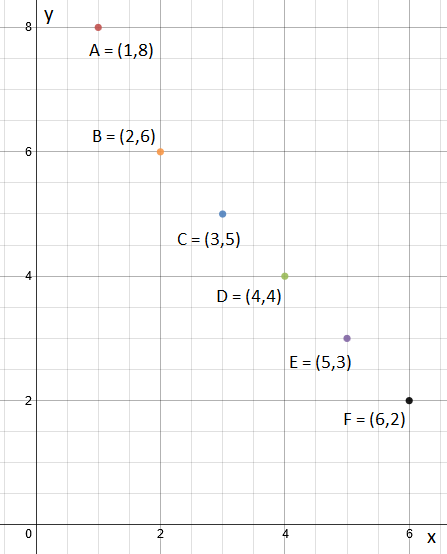
\includegraphics[width=7cm, height=5cm]{EjemploInicialUtil}
  \caption{Puntos distribuidos inicialmente.}
\end{figure}

Primero queremos destruir al objetivo situado en $A$. Miramos el objetivo $B$, que tiene la mayor coordenada $y$ de los que tienen menor coordenada $y$ que $A$ (que son todos dado que se empieza queriendo destruir al objetivo situado en el punto con mayor $y$). En la Figura 2 vemos que $A_{y} > B_{y} + T$ y que A no pertenece al área de impacto A(B, 1), o sea que disparar una genkidama al punto B no eliminaría al androide de A. Por transitividad, como $B_{y} > C_{y} > ... > F_{y}$, ninguno de los disparos a los puntos siguientes a B eliminará al objetivo de A, por lo que es necesario disparar una genkidama a A. El área de impacto A(A, T) = A( (1,8), 1) de esta genkidama, sombrada con rojo en la Figura 2, incluye al punto B, que además es el de mayor coordenada $x$ de los destruidos por esta gendikama.\\
\par{El siguiente a B, C, es el de mayor coordenada $y$ de los que están vivos, y se repite el proceso que se llevó a cabo con A. En la Figura 3 se ve que la segunda gendikama se disparará a D, destruyendo a los objetivos de C, D y E.
Finalmente queda la situación mostrada en la Figura 4 y se dispara una tercera genkidama a F.}\\

\begin{figure}[h!]
\centering
\begin{minipage}{.5\textwidth}
  \centering
  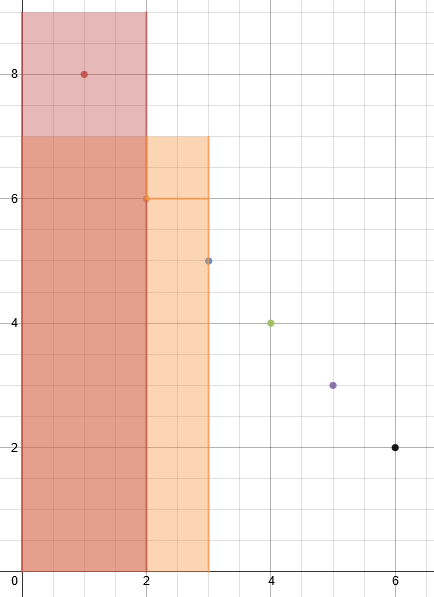
\includegraphics[width=.4\linewidth]{EjemploArea1}
  \caption{Área de impacto de A en rojo y de B en naranja.}
  \label{fig:test1}
\end{minipage}%
\begin{minipage}{.5\textwidth}
  \centering
  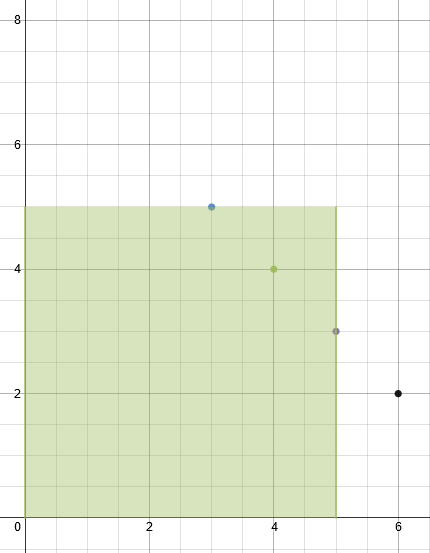
\includegraphics[width=4cm]{EjemploArea2}
  \caption{Área de impacto de D en verde.}
  \label{fig:test2}
\end{minipage}

\end{figure}

\begin{figure}[h!]
\centering
\begin{minipage}{.5\textwidth}
  \centering
  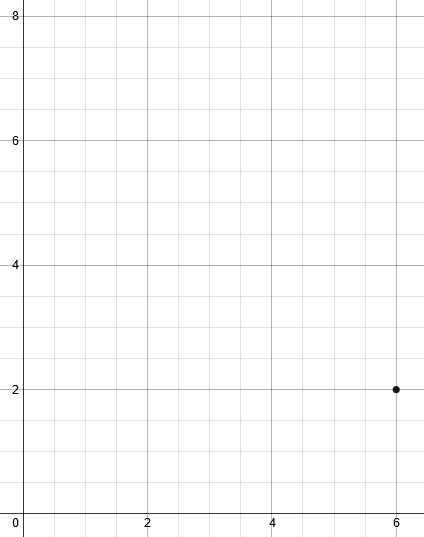
\includegraphics[width=4cm]{EjemploArea3}
  \caption{Androide restante por destruir, en F.}
  \label{fig:test2}
\end{minipage}
\end{figure}

Ahora veamos cómo sería este proceso con $T = 2$.
De vuelta se comienza queriendo destruir al objetivo en A. Como se ve en la Figura 5, disparar a C no destruye a A pero disparar a B sí. Así, morirán los androides situados en los puntos incluidos en la región sombreada naranja en la Figura 6 (el área de impacto A(B, 2)).
\par{Finalmente queda la situación mostrada en la Figura 7 en la que el objetivo es destruir al objetivo de E y se terminará disparando a F eliminando a los dos androides restantes.}
\par{En este caso se habrá destruido a todos los androides utilizando dos genkidamas.}\\

\begin{figure}[h!]
\centering
\begin{minipage}{.5\textwidth}
  \centering
  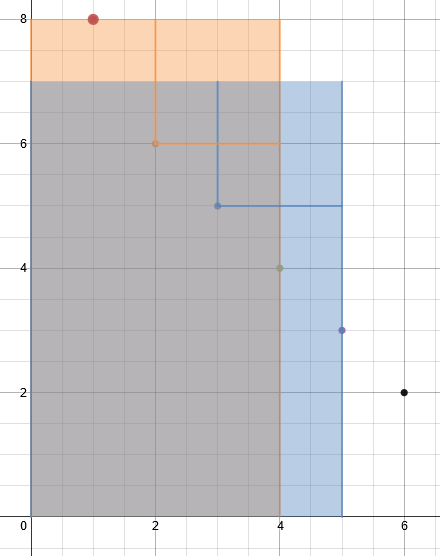
\includegraphics[width=.4\linewidth]{EjemploArea4}
  \caption{Área de impacto de B en naranja y de C en azul.}
  \label{fig:test1}
\end{minipage}%
\begin{minipage}{.5\textwidth}
  \centering
  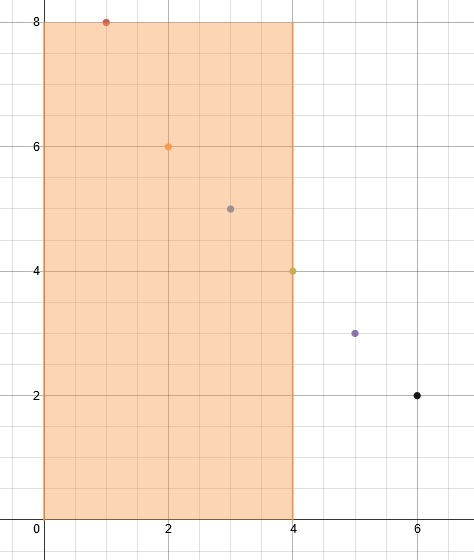
\includegraphics[width=4cm]{EjemploArea5}
  \caption{Área de impacto de B en naranja.}
  \label{fig:test2}
\end{minipage}

\begin{minipage}{.5\textwidth}
  \centering
  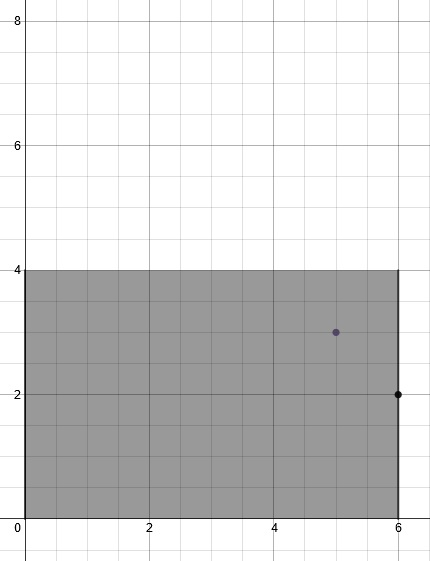
\includegraphics[width=4cm]{EjemploArea6}
  \caption{Área de impacto de F en negro.}
  \label{fig:test2}
\end{minipage}

\end{figure}

\newpage
\subsection{Pseudocódigo}
\begin{algorithm}[h!]
\caption{IndiceDeMenorYQueLoMata}
\begin{algorithmic}
  \Function{IndiceDeMenorYQueLoMata}{t: int, indiceDeObjetivo: int, e: $Arreglo<Tupla<int,int>>$} $\to j$ : \texttt{int}
	\State $int~ j \gets indiceDeObjetivo - 1$ \Comment $\mathcal{O}(1)$
	\While{$(j \geq 0) \wedge (((e[j]).y + t) \geq (e[indiceDeObjetivo]).y)$} \Comment $\mathcal{O}(indiceDeObjetivo)$
		\State j-~- \Comment $\mathcal{O}(1)$
	\EndWhile
	\State j++ \Comment $\mathcal{O}(1)$
	\State return j \Comment $\mathcal{O}(1)$
\EndFunction
\end{algorithmic}
\underline{Complejidad:} $\mathcal{O}(indiceDeObjetivo)$\\
    
\end{algorithm}

\begin{algorithm}[h!]
\caption{IndiceDeMayorXQueMata}
\begin{algorithmic}
  \Function{IndiceDeMayorXQueMata}{t: int, indiceDeObjetivo: int, e: $Arreglo<Tupla<int,int>>$} $\to j$ : \texttt{int}
  	\State $int~ distanciaDeDano \gets e[indiceDeObjetivo].x + t$ \Comment $\mathcal{O}(1)$
	\State $int~ i \gets indiceDeObjetivo - 1$ \Comment $\mathcal{O}(1)$
	\While{$(i \geq 0) \wedge (((e[i]).x) \leq distanciaDeDano$} \Comment $\mathcal{O}(indiceDeObjetivo)$
		\State i-~- \Comment $\mathcal{O}(1)$
	\EndWhile
	\State i++ \Comment $\mathcal{O}(1)$
	\State return i \Comment $\mathcal{O}(1)$
\EndFunction
\end{algorithmic}
\underline{Complejidad:} $\mathcal{O}(indiceDeObjetivo)$\\
    
\end{algorithm}

\begin{algorithm}[h!]
\caption{Genkidama}
\begin{algorithmic}
  \Function{Genkidama}{t: int, n: int, e: $Arreglo<Tupla<int,int>>$}
  	\State $int~[~]~ atacados$ \Comment $\mathcal{O}(1)$
  	\State $int ~genkidamasUtilizadas \gets 0$ \Comment $\mathcal{O}(1)$
	\State $int ~indiceDeObjetivoPorArea \gets n - 1$ \Comment $\mathcal{O}(1)$
	\State $ //~el~ de~ arriba~ es~ aquel~ al~ que~ quiero~ que~ le~ llegue~ la~ onda~ expansiva$
	\State $bool ~hayAlgunoVivo \gets true$ \Comment $\mathcal{O}(1)$
	\While{$hayAlgunoVivo$} \Comment $\mathcal{O}(menorY)$
		\State $ 	//~el~ de~ abajo ~es~ aquel~ al~ que~ le~ voy~ a ~tirar~ la~ bomba$
		\State $int~menorY \gets indiceDeMenorYQueLoMata(t, indiceDeObjetivoPorArea, e)$ \Comment $\mathcal{O}(indiceDeObjetivoPorArea)$
		\State $agregarAtras(atacados, indiceDeObjetivo + 1)$ \Comment $\mathcal{O}(1)$
		\State $		//~el +1 ~de~ arriba~ surge~ de~ que~ en~ el~ enunciado ~se~ enumeran~ desde~ el~ 1 ~$
		\State $	   y~ nosotros~ enumeramos~ desde~ 0$
		\State  $int~indiceDeMayorXMatado \gets indiceDeMayorXQueMata(t, menorY, e)$ \Comment $\mathcal{O}(menorY)$
		\State $hayAlgunoVivo \gets \neg(indiceDeMayorXMatado == 0)$ \Comment $\mathcal{O}(1)$
		\State $indiceDeObjetivoPorArea \gets indiceDeMayorXMatado - 1$ \Comment $\mathcal{O}(1)$
		\State genkidamasUtilizadas++ \Comment $\mathcal{O}(1)$
	\EndWhile
	\State $imprimir ~genkidamasUtilizadas$
	\State $int~ h \gets 0$
	\While{$h < genkidamasUtilizadas$}
			\State $imprimir ~atacados[h]$
			\State $h++$
			\If{$h < genkidamasUtilizadas$}
					\State $imprimir ~"~"~$
			\EndIf
	\EndWhile
\EndFunction
\end{algorithmic}
\underline{Complejidad:} $\mathcal{O}(n)$\\
\\
\underline{Justificación:} 
\end{algorithm}

\par{Teniendo en cuenta que\\
\begin{itemize}
\item[•]$int~menorY \gets indiceDeMenorYQueLoMata(t, indiceDeObjetivoPorArea, e)$ es $\mathcal{O}(indiceDeObjetivoPorArea - menorY + 1)$
\item[•]$int~indiceDeMayorXMatado \gets indiceDeMayorXQueMata(t, indiceDeObjetivo, e)$  es $\mathcal{O}(indiceDeObjetivo - indiceDeMayorXMatado + 1)$
\item[•] y que si notamos\\
$indiceDeObjetivoPorArea_{i}$ a indiceDeObjetivoPorArea al comienzo de la iteración i,\\
$indiceDeMayorXMatado_{i}$ a indiceDeMayorXMatado luego de la asignación realizada en la iteración i,\\
$menorY_{i}$ a menorY luego de la asignación realizada en la iteración i,
\\entonces se tiene
\begin{equation}
indiceDeObjetivoPorArea_{i+1} = indiceDeMayorXMatado_{i} - 1
\end{equation}
\end{itemize}
el cálculo de la complejidad se simplifica.}\\
\par{
Cada iteración i tiene complejidad
\begin{multline}
\mathcal{O}(indiceDeObjetivoPorArea_{i} - menorY_{i} + 1) + \mathcal{O}(menorY_{i} - indiceDeMayorXMatado_{i} + 1)
\\
= \mathcal{O}(indiceDeObjetivoPorArea_{i} - indiceDeMayorXMatado_{i} + 2)
\end{multline}
Para la primera iteración se tiene \\
\begin{equation}
indiceDeObjetivoPorArea_{1} = n-1
\end{equation}
y para la $\acute{u}$ltima se tiene \\
\begin{equation}
indiceDeMayorXMatado_{\#iteraciones} = 0
\end{equation}
Así, la complejidad total del algoritmo es la suma sobre las iteraciones de la complejidad para cada iteración:
}

\begin{multline}
\sum\limits_{i=1}^{\#iteraciones} \mathcal{O}(indicePorArea_{i} - MayorXMatado_{i} + 2)
\\
= \mathcal{O}(indicePorArea_{1} - MayorXMatado_{1} + 2)
\\ + \sum\limits_{i=2}^{\#iteraciones-1} \mathcal{O}(indicePorArea_{i} - MayorXMatado_{i} + 2)
\\ + \mathcal{O}(indicePorArea_{\#iteraciones} - MayorXMatado_{\#iteraciones} + 2)
\\
= \mathcal{O}(n-1) + \sum\limits_{i=1}^{\#iteraciones-1} \mathcal{O}(- MayorXMatado_{i} + 2 + indicePorArea_{i+1}) + \mathcal{O}(0 + 2) 
\\
= \mathcal{O}(n) + \sum\limits_{i=1}^{\#iteraciones-1} \mathcal{O}(- MayorXMatado_{i} + 2 + (MayorXMatado_{i} - 1) )
\\
= \mathcal{O}(n) + \mathcal{O}(\#iteraciones-1) = \mathcal{O}(n) + \mathcal{O}(n)
\\
= \mathcal{O}(n)
\end{multline}


Como se puede ver en el pseudocódigo y se explica en la sección $"$Ideas para desarrollar el algoritmo$"$ se recorren todos los puntos ordenados, de mayor a menor coordenada $y$, una vez, ya sea para encontrar a que enemigo atacar o para ver cuales murieron en el último ataque.\\
Cuando se busca un enemigo a atacar, se verifica que al atacarlo se maten todos los anteriores, así al lanzar una Genkidama sabemos que todos los enemigos por los que ya iteramos estarán muertos y solo queda ver cuales de los siguentes al enemigo atacado tambíen muerieron. Esto se logra iterando por los enemigos subsiguientes al atacado hasta encontrar el primero al que la Genkidama no mató y con él se vuelve a comenzar el proceso. Se puede ver claramente que se itera por todos los enemigos y que se hace solo una vez haciendo que la complejidad sea $\mathcal{O}(n)$ siendo $n$ la cantidad de enemigos.
    



\subsection{Análisis de complejidad}
Como ya se ha explicado, el algoritmo Genkidama tiene complejidad temporal $\mathcal{O}(n)$, pero también podemos afirmar que tiene complejidad temporal $\mathcal{\theta}(n)$ porque para cada androide chequea o  bien si la genkidama tirada en esa ubicación mata a otro o bien si su ubicación es alcanzada por otra explosión. Esto da una cantidad de chequeos de al menos n pues hay n androides.
\par{El mejor caso se tiene cuando todos los androides mueren con una sola genkidama utilizada pues luego de fijar un objetivo sólo se realiza un chequeo para cada uno de los $n-1$ androides.}
\par{El peor caso se tiene cuando para matar a cada androide se requiere una genkidama distinta y por tanto se hacen dos chequeos para destruir cada uno de los $n-1$ androides.}

\newpage
\subsection{Experimentación}
Para la experimentación medimos los tiempos de ejecución para distintos tamaños de entrada y lo hicimos varias veces para cada tamaño de entrada para tener resultados más confiables. Este proceso lo realizamos para las situaciones que creíamos que daban lugar a mejor y peor caso y verificamos que efectivamente eran las situaciones que pensábamos.
\par{Además hicimos un generador de instancias aleatorias y medimos los tiempos de ejecución para muchas entradas generadas aleatoriamente y efectivamente eran tiempos para tamaños de entrada grandes solían estar comprendidos entre los tiempos de ejecución para mejor caso y para peor caso.}
\par{A continuación se exponen la tabla y el gráfico resultante de esas mediciones}\\

\begin{table}[h!]
\centering
\label{my-label}
\begin{tabular}{cc}
\hline
\multicolumn{1}{|c|}{n (Tamaño de la entrada)} & \multicolumn{1}{c|}{Tiempo promedio (nanosegundos)} \\ \hline
\multicolumn{1}{|c|}{10000}                        & \multicolumn{1}{c|}{1245}         \\ \hline
\multicolumn{1}{|c|}{15000}                        & \multicolumn{1}{c|}{1502}         \\ \hline
\multicolumn{1}{|c|}{20000}                        & \multicolumn{1}{c|}{2024}         \\ \hline
\multicolumn{1}{|c|}{25000}                        & \multicolumn{1}{c|}{2582}         \\ \hline
\multicolumn{1}{|c|}{30000}                        & \multicolumn{1}{c|}{3082}         \\ \hline
\multicolumn{1}{|c|}{35000}                        & \multicolumn{1}{c|}{3614}         \\ \hline
\multicolumn{1}{|c|}{40000}                        & \multicolumn{1}{c|}{4433}         \\ \hline
\multicolumn{1}{|c|}{45000}                        & \multicolumn{1}{c|}{5056}         \\ \hline
\multicolumn{1}{|c|}{50000}                        & \multicolumn{1}{c|}{5246}         \\ \hline
\multicolumn{1}{|c|}{55000}                        & \multicolumn{1}{c|}{5954}         \\ \hline
\multicolumn{1}{|c|}{60000}                        & \multicolumn{1}{c|}{6505}         \\ \hline
\multicolumn{1}{|c|}{65000}                        & \multicolumn{1}{c|}{6346}         \\ \hline
\multicolumn{1}{|c|}{70000}                        & \multicolumn{1}{c|}{6816}         \\ \hline
\multicolumn{1}{|c|}{75000}                        & \multicolumn{1}{c|}{7065}         \\ \hline
\multicolumn{1}{|c|}{80000}                        & \multicolumn{1}{c|}{7951}         \\ \hline
\multicolumn{1}{|c|}{85000}                        & \multicolumn{1}{c|}{8516}         \\ \hline
\multicolumn{1}{|c|}{90000}                        & \multicolumn{1}{c|}{9463}         \\ \hline
\multicolumn{1}{|c|}{95000}                        & \multicolumn{1}{c|}{10662}         \\ \hline
\multicolumn{1}{|c|}{100000}                        & \multicolumn{1}{c|}{11851}         \\ \hline
\end{tabular}
\caption{Tabla que muestra los tiempos de ejecución promedio correspondientes a distintos tamaños de entrada con T aleatorio entre cada rango de valores.}
\end{table}

\begin{figure}[h!]
  \centering
  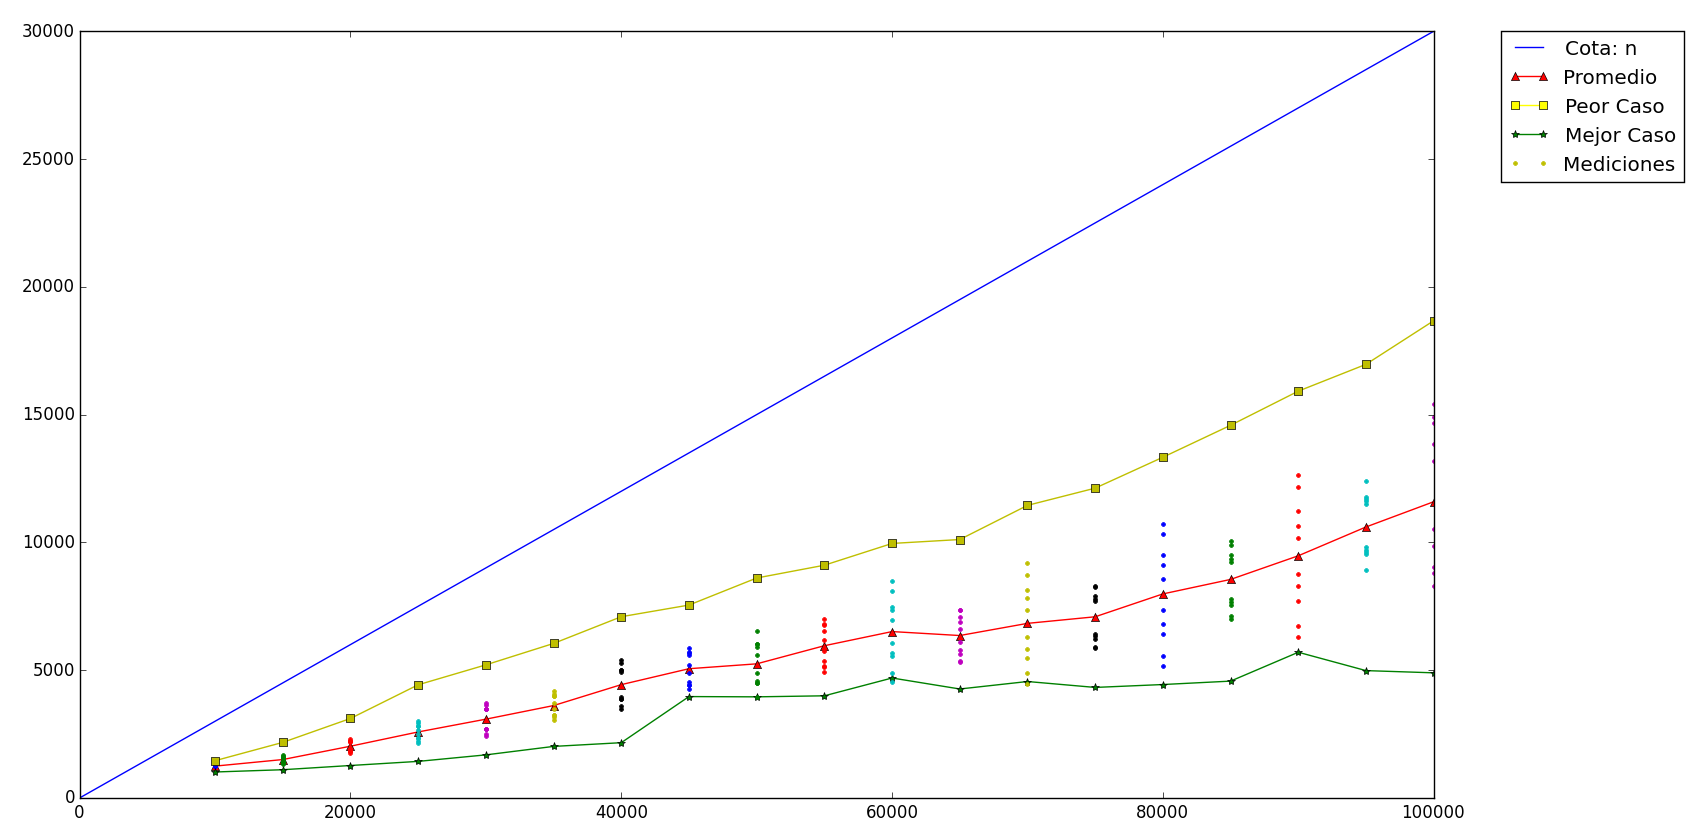
\includegraphics[width=12cm, height=9cm]{tiemposEj2Nuevos}
  \caption{Tiempos de ejecución para distintas entradas. La curva azul es la curva de la complejidad, $0.3*n$ (la constante se incluyó para lograr mostrar claramente que efectivamente el algoritmo es $\mathcal{O}(n)$), la línea verde es mejor caso, la roja caso aleatorio y la amarilla peor caso.}
\end{figure}

\newpage
\subsection{Apéndice: código de Genkidama}
\begin{lstlisting}
#include <tuple>
#include <vector>
#include <iostream>
#include <cassert>
using namespace std;

void genkidama(int, int, vector<tuple<int, int>>);
int indiceDeMenorYQueLoMata(int, int, vector<tuple<int,int>>);
int indiceDeMayorXQueMata(int, int, vector<tuple<int,int>>);

int main(){
	int t;
	int n;
	cin >> n >> t;
	vector<tuple<int,int>> e;
	tuple<int,int> en;
	int x;
	int y;
	for (int i = 0; i < n; i++) {
		cin >> x >> y;
		en = make_tuple(x,y);
		e.push_back((en));
	}
	genkidama(t, n, e);
	return 0;
}

// Toma el t, el indice del objetivo en e y el vector de tuplas.
int indiceDeMenorYQueLoMata(int t, int indiceDeObjetivo, vector<tuple<int,int>> e){
	int j = indiceDeObjetivo - 1;
	while((j >= 0) && ((get<1>(e[j]) + t) >= get<1>(e[indiceDeObjetivo]))){
		j--;
	}
	j++;
	return j;
}

int indiceDeMayorXQueMata(int t, int indiceDeObjetivo, vector<tuple<int,int>> e){
	int distanciaDeDano = get<0>(e[indiceDeObjetivo]) + t;
	int i = indiceDeObjetivo - 1;
	while((i >= 0) && (get<0>(e[i]) <= distanciaDeDano)){
		i--;
	}
	i++;
	return i;
}

void genkidama(int t, int n, vector<tuple<int,int>> e){
	assert (n > 0 && n == e.size() && "La cantidad de enemigos es distinta a la cantidad de posisciones");
	vector<int> atacados;
	int genkidamasUtilizadas = 0;
	int indiceDeObjetivoPorArea = n-1;
	// el de arriba es aquel al que quiero que le llegue la onda expansiva
	bool hayAlgunoVivo = true;
	while(hayAlgunoVivo){
		// el de abajo es aquel al que le voy a tirar la bomba
		int indiceDeObjetivo = indiceDeMenorYQueLoMata(t, indiceDeObjetivoPorArea, e);
		atacados.push_back(indiceDeObjetivo + 1);
		// el +1 de arriba surge de que en el enunciado se enumeran desde el 1 y
		// nosotros enumeramos desde 0
		hayAlgunoVivo = !(indiceDeMayorXQueMata(t, indiceDeObjetivo, e) == 0);
		indiceDeObjetivoPorArea = indiceDeMayorXQueMata(t, indiceDeObjetivo, e) - 1;
		genkidamasUtilizadas++;
		
	}
	std::cout << genkidamasUtilizadas << std::endl;
	int h = 0;
	while (h < genkidamasUtilizadas) {
			std::cout << atacados[h];
			h++;
			if (h < genkidamasUtilizadas) {
					std::cout << " ";
			}
	}
	std::cout << std::endl;
}

\end{lstlisting}
